% Created by tikzDevice version 0.12.3 on 2020-01-31 11:45:38
% !TEX encoding = UTF-8 Unicode
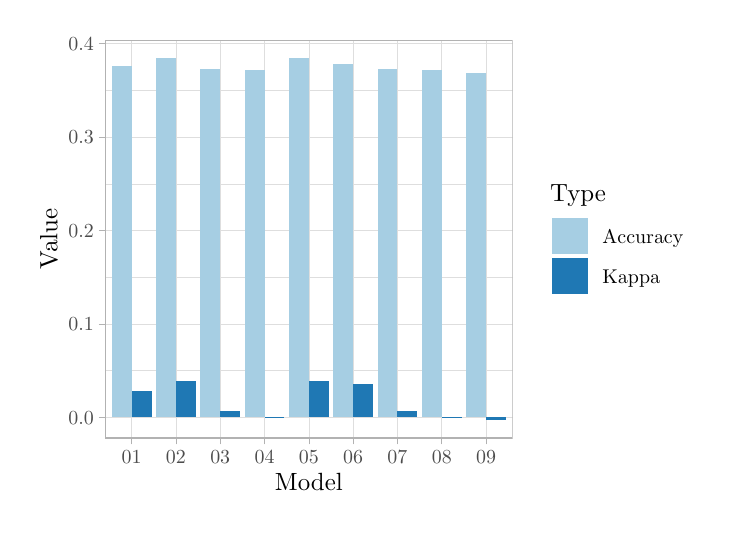
\begin{tikzpicture}[x=1pt,y=1pt]
\definecolor{fillColor}{RGB}{255,255,255}
\path[use as bounding box,fill=fillColor,fill opacity=0.00] (0,0) rectangle (245.72,173.45);
\begin{scope}
\path[clip] (  0.00,  0.00) rectangle (245.72,173.45);
\definecolor{drawColor}{RGB}{255,255,255}
\definecolor{fillColor}{RGB}{255,255,255}

\path[draw=drawColor,line width= 0.5pt,line join=round,line cap=round,fill=fillColor] (  0.00,  0.00) rectangle (245.72,173.45);
\end{scope}
\begin{scope}
\path[clip] ( 27.95, 25.11) rectangle (175.25,168.95);
\definecolor{fillColor}{RGB}{255,255,255}

\path[fill=fillColor] ( 27.95, 25.11) rectangle (175.25,168.95);
\definecolor{drawColor}{gray}{0.87}

\path[draw=drawColor,line width= 0.1pt,line join=round] ( 27.95, 49.52) --
	(175.25, 49.52);

\path[draw=drawColor,line width= 0.1pt,line join=round] ( 27.95, 83.27) --
	(175.25, 83.27);

\path[draw=drawColor,line width= 0.1pt,line join=round] ( 27.95,117.02) --
	(175.25,117.02);

\path[draw=drawColor,line width= 0.1pt,line join=round] ( 27.95,150.78) --
	(175.25,150.78);

\path[draw=drawColor,line width= 0.2pt,line join=round] ( 27.95, 32.64) --
	(175.25, 32.64);

\path[draw=drawColor,line width= 0.2pt,line join=round] ( 27.95, 66.39) --
	(175.25, 66.39);

\path[draw=drawColor,line width= 0.2pt,line join=round] ( 27.95,100.15) --
	(175.25,100.15);

\path[draw=drawColor,line width= 0.2pt,line join=round] ( 27.95,133.90) --
	(175.25,133.90);

\path[draw=drawColor,line width= 0.2pt,line join=round] ( 27.95,167.66) --
	(175.25,167.66);

\path[draw=drawColor,line width= 0.2pt,line join=round] ( 37.55, 25.11) --
	( 37.55,168.95);

\path[draw=drawColor,line width= 0.2pt,line join=round] ( 53.56, 25.11) --
	( 53.56,168.95);

\path[draw=drawColor,line width= 0.2pt,line join=round] ( 69.58, 25.11) --
	( 69.58,168.95);

\path[draw=drawColor,line width= 0.2pt,line join=round] ( 85.59, 25.11) --
	( 85.59,168.95);

\path[draw=drawColor,line width= 0.2pt,line join=round] (101.60, 25.11) --
	(101.60,168.95);

\path[draw=drawColor,line width= 0.2pt,line join=round] (117.61, 25.11) --
	(117.61,168.95);

\path[draw=drawColor,line width= 0.2pt,line join=round] (133.62, 25.11) --
	(133.62,168.95);

\path[draw=drawColor,line width= 0.2pt,line join=round] (149.63, 25.11) --
	(149.63,168.95);

\path[draw=drawColor,line width= 0.2pt,line join=round] (165.64, 25.11) --
	(165.64,168.95);
\definecolor{fillColor}{RGB}{31,120,180}

\path[fill=fillColor] ( 37.55, 32.64) rectangle ( 44.76, 42.28);
\definecolor{fillColor}{RGB}{166,206,227}

\path[fill=fillColor] ( 30.35, 32.64) rectangle ( 37.55,159.65);
\definecolor{fillColor}{RGB}{31,120,180}

\path[fill=fillColor] ( 53.56, 32.64) rectangle ( 60.77, 45.72);
\definecolor{fillColor}{RGB}{166,206,227}

\path[fill=fillColor] ( 46.36, 32.64) rectangle ( 53.56,162.41);
\definecolor{fillColor}{RGB}{31,120,180}

\path[fill=fillColor] ( 69.58, 32.64) rectangle ( 76.78, 35.11);
\definecolor{fillColor}{RGB}{166,206,227}

\path[fill=fillColor] ( 62.37, 32.64) rectangle ( 69.58,158.61);
\definecolor{fillColor}{RGB}{31,120,180}

\path[fill=fillColor] ( 85.59, 32.35) rectangle ( 92.79, 32.64);
\definecolor{fillColor}{RGB}{166,206,227}

\path[fill=fillColor] ( 78.38, 32.64) rectangle ( 85.59,158.27);
\definecolor{fillColor}{RGB}{31,120,180}

\path[fill=fillColor] (101.60, 32.64) rectangle (108.80, 45.72);
\definecolor{fillColor}{RGB}{166,206,227}

\path[fill=fillColor] ( 94.39, 32.64) rectangle (101.60,162.41);
\definecolor{fillColor}{RGB}{31,120,180}

\path[fill=fillColor] (117.61, 32.64) rectangle (124.82, 44.81);
\definecolor{fillColor}{RGB}{166,206,227}

\path[fill=fillColor] (110.40, 32.64) rectangle (117.61,160.34);
\definecolor{fillColor}{RGB}{31,120,180}

\path[fill=fillColor] (133.62, 32.64) rectangle (140.83, 35.11);
\definecolor{fillColor}{RGB}{166,206,227}

\path[fill=fillColor] (126.42, 32.64) rectangle (133.62,158.61);
\definecolor{fillColor}{RGB}{31,120,180}

\path[fill=fillColor] (149.63, 32.35) rectangle (156.84, 32.64);
\definecolor{fillColor}{RGB}{166,206,227}

\path[fill=fillColor] (142.43, 32.64) rectangle (149.63,158.27);
\definecolor{fillColor}{RGB}{31,120,180}

\path[fill=fillColor] (165.64, 31.64) rectangle (172.85, 32.64);
\definecolor{fillColor}{RGB}{166,206,227}

\path[fill=fillColor] (158.44, 32.64) rectangle (165.64,156.89);
\definecolor{drawColor}{gray}{0.70}

\path[draw=drawColor,line width= 0.5pt,line join=round,line cap=round] ( 27.95, 25.11) rectangle (175.25,168.95);
\end{scope}
\begin{scope}
\path[clip] (  0.00,  0.00) rectangle (245.72,173.45);
\definecolor{drawColor}{gray}{0.30}

\node[text=drawColor,anchor=base east,inner sep=0pt, outer sep=0pt, scale=  0.72] at ( 23.90, 30.16) {0.0};

\node[text=drawColor,anchor=base east,inner sep=0pt, outer sep=0pt, scale=  0.72] at ( 23.90, 63.91) {0.1};

\node[text=drawColor,anchor=base east,inner sep=0pt, outer sep=0pt, scale=  0.72] at ( 23.90, 97.67) {0.2};

\node[text=drawColor,anchor=base east,inner sep=0pt, outer sep=0pt, scale=  0.72] at ( 23.90,131.42) {0.3};

\node[text=drawColor,anchor=base east,inner sep=0pt, outer sep=0pt, scale=  0.72] at ( 23.90,165.18) {0.4};
\end{scope}
\begin{scope}
\path[clip] (  0.00,  0.00) rectangle (245.72,173.45);
\definecolor{drawColor}{gray}{0.70}

\path[draw=drawColor,line width= 0.2pt,line join=round] ( 25.70, 32.64) --
	( 27.95, 32.64);

\path[draw=drawColor,line width= 0.2pt,line join=round] ( 25.70, 66.39) --
	( 27.95, 66.39);

\path[draw=drawColor,line width= 0.2pt,line join=round] ( 25.70,100.15) --
	( 27.95,100.15);

\path[draw=drawColor,line width= 0.2pt,line join=round] ( 25.70,133.90) --
	( 27.95,133.90);

\path[draw=drawColor,line width= 0.2pt,line join=round] ( 25.70,167.66) --
	( 27.95,167.66);
\end{scope}
\begin{scope}
\path[clip] (  0.00,  0.00) rectangle (245.72,173.45);
\definecolor{drawColor}{gray}{0.70}

\path[draw=drawColor,line width= 0.2pt,line join=round] ( 37.55, 22.86) --
	( 37.55, 25.11);

\path[draw=drawColor,line width= 0.2pt,line join=round] ( 53.56, 22.86) --
	( 53.56, 25.11);

\path[draw=drawColor,line width= 0.2pt,line join=round] ( 69.58, 22.86) --
	( 69.58, 25.11);

\path[draw=drawColor,line width= 0.2pt,line join=round] ( 85.59, 22.86) --
	( 85.59, 25.11);

\path[draw=drawColor,line width= 0.2pt,line join=round] (101.60, 22.86) --
	(101.60, 25.11);

\path[draw=drawColor,line width= 0.2pt,line join=round] (117.61, 22.86) --
	(117.61, 25.11);

\path[draw=drawColor,line width= 0.2pt,line join=round] (133.62, 22.86) --
	(133.62, 25.11);

\path[draw=drawColor,line width= 0.2pt,line join=round] (149.63, 22.86) --
	(149.63, 25.11);

\path[draw=drawColor,line width= 0.2pt,line join=round] (165.64, 22.86) --
	(165.64, 25.11);
\end{scope}
\begin{scope}
\path[clip] (  0.00,  0.00) rectangle (245.72,173.45);
\definecolor{drawColor}{gray}{0.30}

\node[text=drawColor,anchor=base,inner sep=0pt, outer sep=0pt, scale=  0.72] at ( 37.55, 16.10) {01};

\node[text=drawColor,anchor=base,inner sep=0pt, outer sep=0pt, scale=  0.72] at ( 53.56, 16.10) {02};

\node[text=drawColor,anchor=base,inner sep=0pt, outer sep=0pt, scale=  0.72] at ( 69.58, 16.10) {03};

\node[text=drawColor,anchor=base,inner sep=0pt, outer sep=0pt, scale=  0.72] at ( 85.59, 16.10) {04};

\node[text=drawColor,anchor=base,inner sep=0pt, outer sep=0pt, scale=  0.72] at (101.60, 16.10) {05};

\node[text=drawColor,anchor=base,inner sep=0pt, outer sep=0pt, scale=  0.72] at (117.61, 16.10) {06};

\node[text=drawColor,anchor=base,inner sep=0pt, outer sep=0pt, scale=  0.72] at (133.62, 16.10) {07};

\node[text=drawColor,anchor=base,inner sep=0pt, outer sep=0pt, scale=  0.72] at (149.63, 16.10) {08};

\node[text=drawColor,anchor=base,inner sep=0pt, outer sep=0pt, scale=  0.72] at (165.64, 16.10) {09};
\end{scope}
\begin{scope}
\path[clip] (  0.00,  0.00) rectangle (245.72,173.45);
\definecolor{drawColor}{RGB}{0,0,0}

\node[text=drawColor,anchor=base,inner sep=0pt, outer sep=0pt, scale=  0.90] at (101.60,  6.25) {Model};
\end{scope}
\begin{scope}
\path[clip] (  0.00,  0.00) rectangle (245.72,173.45);
\definecolor{drawColor}{RGB}{0,0,0}

\node[text=drawColor,rotate= 90.00,anchor=base,inner sep=0pt, outer sep=0pt, scale=  0.90] at ( 10.70, 97.03) {Value};
\end{scope}
\begin{scope}
\path[clip] (  0.00,  0.00) rectangle (245.72,173.45);
\definecolor{fillColor}{RGB}{255,255,255}

\path[fill=fillColor] (184.25, 71.85) rectangle (241.22,122.21);
\end{scope}
\begin{scope}
\path[clip] (  0.00,  0.00) rectangle (245.72,173.45);
\definecolor{drawColor}{RGB}{0,0,0}

\node[text=drawColor,anchor=base west,inner sep=0pt, outer sep=0pt, scale=  0.90] at (188.75,110.63) {Type};
\end{scope}
\begin{scope}
\path[clip] (  0.00,  0.00) rectangle (245.72,173.45);
\definecolor{fillColor}{RGB}{255,255,255}

\path[fill=fillColor] (188.75, 90.80) rectangle (203.21,105.26);
\end{scope}
\begin{scope}
\path[clip] (  0.00,  0.00) rectangle (245.72,173.45);
\definecolor{fillColor}{RGB}{166,206,227}

\path[fill=fillColor] (189.46, 91.51) rectangle (202.49,104.55);
\end{scope}
\begin{scope}
\path[clip] (  0.00,  0.00) rectangle (245.72,173.45);
\definecolor{fillColor}{RGB}{255,255,255}

\path[fill=fillColor] (188.75, 76.35) rectangle (203.21, 90.80);
\end{scope}
\begin{scope}
\path[clip] (  0.00,  0.00) rectangle (245.72,173.45);
\definecolor{fillColor}{RGB}{31,120,180}

\path[fill=fillColor] (189.46, 77.06) rectangle (202.49, 90.09);
\end{scope}
\begin{scope}
\path[clip] (  0.00,  0.00) rectangle (245.72,173.45);
\definecolor{drawColor}{RGB}{0,0,0}

\node[text=drawColor,anchor=base west,inner sep=0pt, outer sep=0pt, scale=  0.72] at (207.71, 95.55) {Accuracy};
\end{scope}
\begin{scope}
\path[clip] (  0.00,  0.00) rectangle (245.72,173.45);
\definecolor{drawColor}{RGB}{0,0,0}

\node[text=drawColor,anchor=base west,inner sep=0pt, outer sep=0pt, scale=  0.72] at (207.71, 81.10) {Kappa};
\end{scope}
\end{tikzpicture}
